% SPDX-License-Identifier: BSD-2-Clause
%
% Copyright (C) 2026 embedded brains GmbH & Co. KG
%
% Redistribution and use in source and binary forms, with or without
% modification, are permitted provided that the following conditions
% are met:
% 1. Redistributions of source code must retain the above copyright
%    notice, this list of conditions and the following disclaimer.
% 2. Redistributions in binary form must reproduce the above copyright
%    notice, this list of conditions and the following disclaimer in the
%    documentation and/or other materials provided with the distribution.
%
% THIS SOFTWARE IS PROVIDED BY THE COPYRIGHT HOLDERS AND CONTRIBUTORS "AS IS"
% AND ANY EXPRESS OR IMPLIED WARRANTIES, INCLUDING, BUT NOT LIMITED TO, THE
% IMPLIED WARRANTIES OF MERCHANTABILITY AND FITNESS FOR A PARTICULAR PURPOSE
% ARE DISCLAIMED. IN NO EVENT SHALL THE COPYRIGHT OWNER OR CONTRIBUTORS BE
% LIABLE FOR ANY DIRECT, INDIRECT, INCIDENTAL, SPECIAL, EXEMPLARY, OR
% CONSEQUENTIAL DAMAGES (INCLUDING, BUT NOT LIMITED TO, PROCUREMENT OF
% SUBSTITUTE GOODS OR SERVICES; LOSS OF USE, DATA, OR PROFITS; OR BUSINESS
% INTERRUPTION) HOWEVER CAUSED AND ON ANY THEORY OF LIABILITY, WHETHER IN
% CONTRACT, STRICT LIABILITY, OR TORT (INCLUDING NEGLIGENCE OR OTHERWISE)
% ARISING IN ANY WAY OUT OF THE USE OF THIS SOFTWARE, EVEN IF ADVISED OF THE
% POSSIBILITY OF SUCH DAMAGE.

\documentclass[tikz,border=4pt]{standalone}
\usepackage[T1]{fontenc}
\usepackage[scaled]{helvet}
\renewcommand{\familydefault}{\sfdefault}
\usetikzlibrary{arrows.meta,positioning,fit,backgrounds,shapes.geometric}
\definecolor{ebblue}{HTML}{1F4E79}
\definecolor{boxfill}{HTML}{EAF1F8}
\definecolor{codefill}{HTML}{FFF4E0}
\definecolor{codeline}{HTML}{9C6500}
\definecolor{groupfill}{HTML}{F5F5F5}
\definecolor{flow}{HTML}{404040}
\newcommand{\code}[1]{{\ttfamily\scriptsize #1}}
\begin{document}
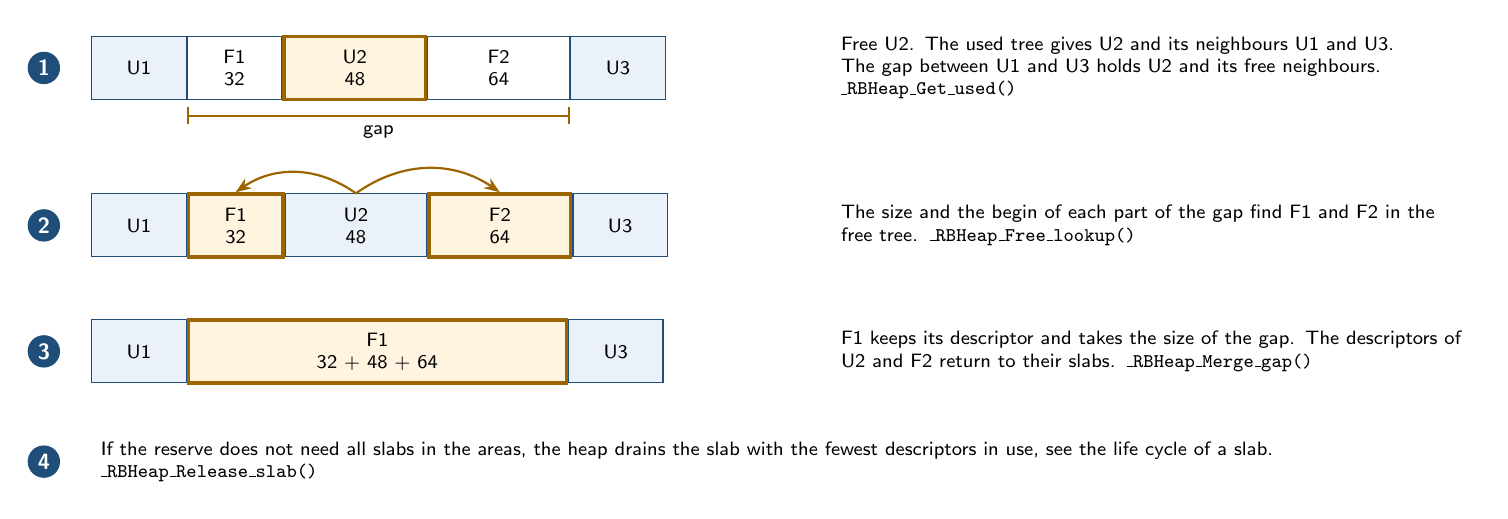
\begin{tikzpicture}[
    font=\small,
    blk/.style={draw=ebblue, minimum height=8mm, align=center,
      font=\scriptsize, inner sep=1pt, anchor=west},
    usedb/.style={blk, fill=boxfill},
    freeb/.style={blk, fill=white},
    hit/.style={blk, fill=codefill, draw=codeline, very thick},
    num/.style={circle, draw=ebblue, fill=ebblue, text=white,
      font=\footnotesize\bfseries, inner sep=1.5pt},
    note/.style={font=\scriptsize, align=left, anchor=west, text width=80mm},
    lockframe/.style={fill=groupfill, draw=gray, rounded corners=3pt},
    gapline/.style={{Bar[]}-{Bar[]}, thick, draw=codeline},
    move/.style={-{Stealth[length=2mm]}, thick, draw=codeline}]
  % 1: used lookup
  \node[num] at (-0.6,0) {1};
  \node[usedb, minimum width=12mm] (a1) at (0,0) {U1};
  \node[freeb, minimum width=12mm] (a2) at (a1.east) {F1\\32};
  \node[hit, minimum width=18mm] (a3) at (a2.east) {U2\\48};
  \node[freeb, minimum width=18mm] (a4) at (a3.east) {F2\\64};
  \node[usedb, minimum width=12mm] (a5) at (a4.east) {U3};
  \draw[gapline] ([yshift=-2mm]a2.south west) -- node[below, font=\scriptsize] {gap} ([yshift=-2mm]a4.south east);
  \node[note] at (9.4,0) {Free U2.  The used tree gives U2 and its
    neighbours U1 and U3.  The gap between U1 and U3 holds U2 and its free
    neighbours.  \code{\_RBHeap\_Get\_used()}};
  % 2: free lookup
  \node[num] at (-0.6,-2.0) {2};
  \node[usedb, minimum width=12mm] (b1) at (0,-2.0) {U1};
  \node[hit, minimum width=12mm] (b2) at (b1.east) {F1\\32};
  \node[usedb, minimum width=18mm] (b3) at (b2.east) {U2\\48};
  \node[hit, minimum width=18mm] (b4) at (b3.east) {F2\\64};
  \node[usedb, minimum width=12mm] (b5) at (b4.east) {U3};
  \draw[move] (b3.north) to[bend right=35] (b2.north);
  \draw[move] (b3.north) to[bend left=35] (b4.north);
  \node[note] at (9.4,-2.0) {The size and the begin of each part of the gap
    find F1 and F2 in the free tree.  \code{\_RBHeap\_Free\_lookup()}};
  % 3: merge
  \node[num] at (-0.6,-3.6) {3};
  \node[usedb, minimum width=12mm] (c1) at (0,-3.6) {U1};
  \node[hit, minimum width=48mm] (c2) at (c1.east) {F1\\32 + 48 + 64};
  \node[usedb, minimum width=12mm] (c3) at (c2.east) {U3};
  \node[note] at (9.4,-3.6) {F1 keeps its descriptor and takes the size of
    the gap.  The descriptors of U2 and F2 return to their slabs.
    \code{\_RBHeap\_Merge\_gap()}};
  % 4: release
  \node[num] at (-0.6,-5.0) {4};
  \node[note, text width=150mm] at (0,-5.0) {If the reserve does not need all
    slabs in the areas, the heap drains the slab with the fewest descriptors in
    use, see the life cycle of a slab.  \code{\_RBHeap\_Release\_slab()}};
\end{tikzpicture}
\end{document}
